\documentclass[letterpaper,12pt,fleqn]{article}
\usepackage{matharticle}
\pagestyle{empty}

\newcommand{\e}{\epsilon}
\renewcommand{\d}{\delta}

\begin{document}

\section*{Limits}

\begin{example}

  Consider the standard function \(f(x)=x^2\):

  \bigskip

  \begin{center}
    \begin{tikzpicture}
      \begin{axis}[
          axis lines=middle,
          xmin=-5,
          xmax=5,
          ymin=-1/2,
          ymax=6,
          ticks=none,
          xlabel={\(x\)},
          ylabel={\(y\)},
          x label style={at={(axis cs:5,0)},anchor=west},
          y label style={at={(axis cs:0,6)},anchor=south},
        ]
        \addplot [domain=-2.5:2.5,blue] {x^2};
        \node [closed point,red] (P) at (2,4) {};
        \draw [dashed] (P) to (2,0) node [below] {\(2\)};
      \end{axis}
    \end{tikzpicture}
  \end{center}

  \bigskip

  What happens to \(f(x)\) as \(x\to2\) (but \(x\ne 2\))?

  \bigskip

  \begin{center}
    \(\begin{array}{|l|l|}
    \hline
    x & f(x) \\
    \hline
    \hline
    2.1 & 4.41 \\
    \hline
    2.01 & 4.0401 \\
    \hline
    2.001 & 4.004001 \\
    \hline
    2.0001 & 4.00040001 \\
    \hline
    2 & ??? \\
    \hline
    1.9999 & 3.99960001 \\
    \hline
    1.999 & 3.996001 \\
    \hline
    1.99 & 3.9601 \\
    \hline
    1.9 & 3.61 \\
    \hline
    \end{array}\)
  \end{center}

  \bigskip

  It appears that \(f(x)\to4\) as \(x\to2\) (from either direction).
\end{example}

In the previous example, it turns out that \(f(x)\) is actually defined at \(x=2\) and furthermore, \(f(2)=4\).
This special case will be used later as a formal definition of \emph{continuity}.  However, as previously stated,
we don't actually care about the function value at \(x=2\).  In fact, the function might not even be defined at the
\(x\) value in question.

\begin{example}
  Consider the rational function:
  \[f(x)=\frac{x^2(x-2)}{x-2}\]

  \begin{center}
    \begin{tikzpicture}
      \begin{axis}[
          axis lines=middle,
          xmin=-5,
          xmax=5,
          ymin=-1/2,
          ymax=6,
          ticks=none,
          xlabel={\(x\)},
          ylabel={\(y\)},
          x label style={at={(axis cs:5,0)},anchor=west},
          y label style={at={(axis cs:0,6)},anchor=south},
        ]
        \addplot [domain=-2.5:2.5,blue] {x^2};
        \node [closed point,fill=white] (P) at (2,4) {};
        \draw [dashed] (P) to (2,0) node [below] {\(2\)};
      \end{axis}
    \end{tikzpicture}
  \end{center}

  \bigskip

  Now, as \(x\to2\), the above table of values still applies and so it appears that \(f(x)\to4\) as \(x\to2\) (from
  either direction) even though \(f(2)\) is not defined.  To reiterate, we do not care what actually happens at
  \(x=2\).  In fact, let's define \(f(2)=1\):
  \[f(x)=\begin{cases}
  \frac{x^2(x-2)}{x-2}, & x\ne2 \\
  1, & x=2
  \end{cases}\]

  \begin{center}
    \begin{tikzpicture}
      \begin{axis}[
          axis lines=middle,
          xmin=-5,
          xmax=5,
          ymin=-1/2,
          ymax=6,
          ticks=none,
          xlabel={\(x\)},
          ylabel={\(y\)},
          x label style={at={(axis cs:5,0)},anchor=west},
          y label style={at={(axis cs:0,6)},anchor=south},
        ]
        \addplot [domain=-2.5:2.5,blue] {x^2};
        \node [closed point,fill=white] (P) at (2,4) {};
        \draw [dashed] (P) to (2,0) node [below] {\(2\)};
        \node [closed point] at (2,1) {};
      \end{axis}
    \end{tikzpicture}
  \end{center}

  \bigskip

  Still, \(f(x)\to4\) as \(x\to2\), regardless of the fact that \(f(2)=1\).  Once again, we do not care about the
  function at \(x=2\); we only care what happens arbitrarily close to \(x=2\).
\end{example}

\begin{example}
  Consider the function:
  \[f(x)=\frac{\sin x}{x}\]

  \bigskip

  \begin{center}
    \begin{tikzpicture}
      \begin{axis}[
          axis lines=middle,
          xmin=-5,
          xmax=5,
          ymin=-2,
          ymax=2,
          ticks=none,
          xlabel={\(x\)},
          ylabel={\(y\)},
          x label style={at={(axis cs:5,0)},anchor=west},
          y label style={at={(axis cs:0,2)},anchor=south},
          clip=false
        ]
        \addplot [domain=-5:5,blue] {(sin(deg(x)))/x};
        \node [closed point,fill=white] at (0,1) {};
      \end{axis}
    \end{tikzpicture}
  \end{center}

  As \(x\to0\):

  \begin{center}
    \(\begin{array}{|l|l|}
    \hline
    x & f(x) \\
    \hline
    \hline
    1 & 0.841471 \\
    \hline
    0.1 & 0.998334 \\
    \hline
    0.01 & 0.999983 \\
    \hline
    0 & ??? \\
    \hline
    -0.01 & 0.999983 \\
    \hline
    -0.1 & 0.998334 \\
    \hline
    -1 & 0.841471 \\
    \hline
    \end{array}\)
  \end{center}

  \bigskip

  It appears that \(f(x)\to1\) as \(x\to0\).
\end{example}

In the previous two examples, when the functions are evaluated at the point in question the result is
\(\frac{0}{0}\), which is one of the so-called \emph{indeterminate forms} \((\frac{0}{0},\frac{\infty}{\infty},
0\cdot\infty,\infty-\infty,1^{\infty})\).  When the resulting form is indeterminate, additional effort is required
to determine the actual behavior arbitrarily close to the point.

\begin{definition}[Limit of a Function at a Point]
  To say that \(L\in\R\) is the \emph{limit} of a function \(f(x)\) at \(x=a\), denoted by
  \(\displaystyle\lim_{x\to a}f(x)=L\), means that \(f(x)\to L\) as \(x\to a\) (but \(x\ne a\)):
  \[\forall\,\e>0,\exists\,\d>0,\forall\,x\in\R,0<\abs{x-a}<\d\implies\abs{f(x)-L}<\e\]
  An alternate syntax is: \(f(x)\to0\) as \(x\to a\); however, note that \(f(x)=L\) is allowed.
\end{definition}

Select an \(\e>0\) and then find a \(\d>0\) such that \(f(x)\) is completely contained in the bounding box
\((a-\d,a+\d)\times(L-\e,L+\e)\).

\bigskip

\begin{center}
  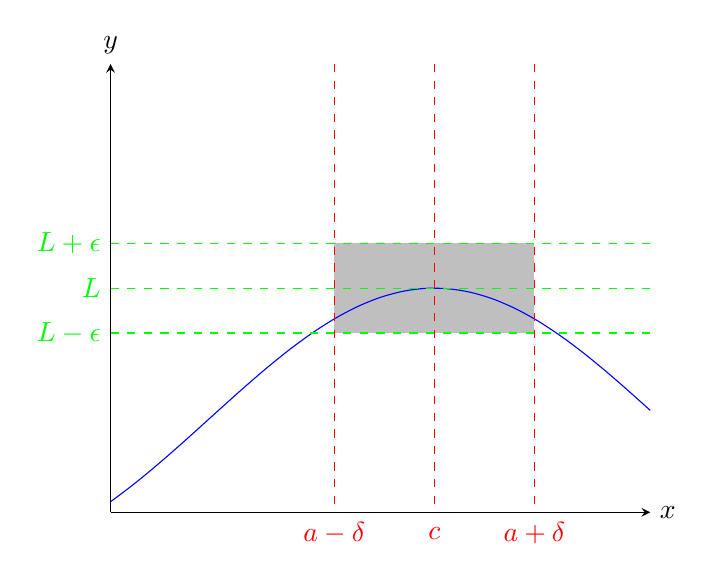
\begin{tikzpicture}
    \begin{axis}[
        axis lines=middle,
        xmin=0,
        xmax=5,
        ymin=0,
        ymax=2,
        ticks=none,
        xlabel={\(x\)},
        ylabel={\(y\)},
        x label style={at={(axis cs:5,0)},anchor=west},
        y label style={at={(axis cs:0,2)},anchor=south},
        clip=false
      ]
      \fill [lightgray] (3-0.9273,0.8) rectangle (3+0.9273,1.2);
      \addplot [domain=0:5,blue,smooth] {(sin(deg(x-3)))/(x-3)};
      \draw [dashed,green] (5,1.2) -- (0,1.2) node [left,green] {\(L+\e\)};
      \draw [dashed,green] (5,1) -- (0,1) node [left,green] {\(L\)};
      \draw [dashed,green] (5,0.8) -- (0,0.8) node [left,green] {\(L-\e\)};
      \draw [dashed,red] (3-0.9273,2) -- (3-0.9273,0) node [below,red] {\(a-\d\)};
      \draw [dashed,red] (3,2) -- (3,0) node [below=0.5ex,red] {\(c\)};
      \draw [dashed,red] (3.9273,2) -- (3.9273,0) node [below,red] {\(a+\d\)};
    \end{axis}
  \end{tikzpicture}
\end{center}

\bigskip

Since this must be the case for all possible \(\e\), as \(\e\to0\) arbitrarily small values of \(\d\) can be
selected such that the bounding box converges on the limit point.

\bigskip

\begin{center}
  \begin{tikzpicture}
    \begin{axis}[
        axis lines=middle,
        xmin=0,
        xmax=5,
        ymin=0,
        ymax=2,
        ticks=none,
        xlabel={\(x\)},
        ylabel={\(y\)},
        x label style={at={(axis cs:5,0)},anchor=west},
        y label style={at={(axis cs:0,2)},anchor=south},
        clip=false
      ]
      \addplot [domain=0:5,blue,smooth] {(sin(deg(x-3)))/(x-3)};
      \draw [dashed,green] (5,1.2) -- (0,1.2) node [left,green] {\(L+\e\)};
      \draw [dashed,green] (5,1) -- (0,1) node [left,green] {\(L\)};
      \draw [dashed,green] (5,0.8) -- (0,0.8) node [left,green] {\(L-\e\)};
      \draw [dashed,red] (3-0.9273,2) -- (3-0.9273,0) node [below,red] {\(a-\d\)};
      \draw [dashed,red] (3,2) -- (3,0) node [below=0.5ex,red] {\(c\)};
      \draw [dashed,red] (3.9273,2) -- (3.9273,0) node [below,red] {\(a+\d\)};
      \draw [blue,very thin] (3-0.9273,0.8) rectangle (3+0.9273,1.2);
      \draw [blue,very thin] (3-0.75,0.85) rectangle (3+0.75,1.15);
      \draw [blue,very thin] (3-0.5,0.9) rectangle (3+0.5,1.1);
      \draw [blue,very thin] (3-0.25,0.95) rectangle (3+0.25,1.05);
      \draw [blue,very thin] (3-0.1,0.98) rectangle (3+0.1,1.02);
    \end{axis}
  \end{tikzpicture}
\end{center}

\bigskip

It is tempting to think that \(\e\to0\) \emph{forces} \(\d\to0\); however, this is not always the case.

\begin{example}
  Consider the constant function \(f(x)=3\) and \(a=2\):

  \bigskip

  \begin{center}
    \begin{tikzpicture}
      \fill [lightgray] (1.25,2.25) rectangle (2.75,3.75);
      \draw [<->] (-1,0) -- (5,0) node [right] {\(x\)};
      \draw [<->] (0,-1) -- (0,5) node [right] {\(y\)};
      \draw [blue] (-1,3) -- (5,3);
      \draw [dashed] (2,3) -- (2,0) node [below] {\(2\)};
      \node [closed point,red] at (2,3) {};
      \draw [dashed, green] (-1,3.75) -- (5,3.75);
      \draw [dashed, green] (-1,2.25) -- (5,2.25);
      \node [above left] at (0,3.75) {\(3+\e\)};
      \node [above left] at (0,2.25) {\(3-\e\)};
      \node [above left] at (0,3) {\(3\)};
      \draw [dashed,red] (1.25,3.75) -- (1.25,0) node [below] {\(2-\d\)};
      \draw [dashed,red] (2.75,3.75) -- (2.75,0) node [below] {\(2+\d\)};
      \node at (8,2.5) {\(\displaystyle\lim_{x\to2}f(x)=3\)};
    \end{tikzpicture}
  \end{center}

  \bigskip

  For any \(\e\), any \(\d\) is sufficient.  Also note that \(f(x)=L\) within every bounding box.
\end{example}

\begin{example}
  Consider the function \(f(x)=x^2+2x-1\) and note that \(\displaystyle\lim_{x\to1}f(x)=2\).  Find a suitable
  \(\d\) to two decimal places for \(\e=0.1\).

  \bigskip

  Although this can be done analytically, the algebra tends to get messy.  A convenient shortcut is to use a
  graphing calculator.  The general procedure is as follows:

  \bigskip

  \begin{enumerate}
  \item Graph the function and mark the \(\e\)-neighborhood around the limit by graphing the constant functions
    \(y=2+0.1=2.1\) and \(y=2-0.1=1.9\).  Adjust the Window so that there is sufficient separation to see all three
    graphs.

    \bigskip

    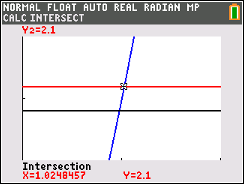
\includegraphics[scale=0.75]{poly01a}\qquad
    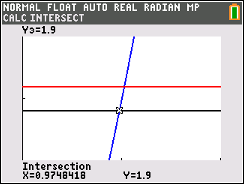
\includegraphics[scale=0.75]{poly01b}

    \bigskip

  \item Use the \emph{intersection} function to determine the minimum and maximum \(x\) values around \(x=1\) such
    that the graph of the function is completely within the marked \(\e\)-neighborhood.
    \begin{gather*}
      x_1=0.9748418 \\
      x_2=1.0248457 \\
      \\
      0.9748418<x<1.0248457
    \end{gather*}
  \item Calculate the distance of each endpoint from \(x=1\):
    \begin{gather*}
      \d_1=1.024845-1=0.0248457 \\
      \d_2=1-0.9748418=0.0251582
    \end{gather*}
  \item Select the smaller of the two distances for \(\d\):
    \[\d=\min\set{\d_1,\d_2}=0.0248457\]
  \item Be sure to round down to stay within the selected interval.
    \[\d=0.024\]
  \end{enumerate}

  Therefore, if \(\abs{x-1}<0.024\) then \(\abs{f(x)-2}<0.1\).

  \bigskip

  Find a suitable \(\d\) to four decimal places for \(\e=0.01\).

  \bigskip

  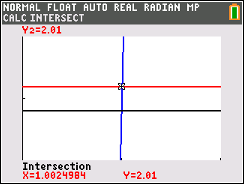
\includegraphics[scale=0.75]{poly001a}\qquad
  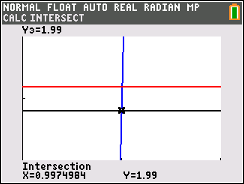
\includegraphics[scale=0.75]{poly001b}

  \begin{gather*}
    \d_1=1.0024984-1=0.0024984 \\
    \d_2=1-0.9974984=0.0025016 \\
    \\
    \d=\min\set{\d_1,\d_2}=0.0024984
  \end{gather*}

  \(\d=0.0024\).

  Therefore, if \(\abs{x-1}<0.0024\) then \(\abs{f(x)-2}<0.01\).
\end{example}

\begin{example}
  Solve the previous problem for \(\e=0.1\) analytically.
  \begin{gather*}
    \abs{f(x)-2}<0.1 \\
    \abs{(x^2+2x-1)-2}<0.1 \\
    \abs{x^2+2x-3}<0.1 \\
    -0.1<x^2+2x-3<0.1 \\
    \\
    x^2+2x-3>-0.1 \\
    x^2+2x-2.9>0 \\
    x=\frac{-2\pm\sqrt{2^2-4(1)(-2.9)}}{2(1)}=-1\pm\sqrt{3.9} \\
    x=-2.9748,0.9748 \\
    0^2+2(0)-2.9=-2.9<0 \\
    x\in(-\infty,-2.9748)\cup(0.9748,\infty) \\
    \\
    x^2+2x-3<0.1 \\
    x^2+2x-3.1<0 \\
    x=\frac{-2\pm\sqrt{2^2-4(1)(-3.1)}}{2(1)}=-1\pm\sqrt{4.1} \\
    x=-3.0248,1.0248 \\
    0^2+2(0)-3.1=-3.1<0 \\
    x\in(-3.0248,1.0248) \\
    \\
    x\in((-\infty,-2.9748)\cup(0.9748,\infty))\cap(-3.0248,1.0248)
  \end{gather*}
  \begin{center}
    \begin{tikzpicture}
      \draw [<->] (-5,0) -- (5,0);
      \node (A) [open point] at (-4,0) {};
      \node [below] at (A) {\(-3.0248\)};
      \node (B) [open point] at (-2,0) {};
      \node [below] at (B) {\(-2.9748\)};
      \node (C) [open point] at (2,0) {};
      \node [below] at (C) {\(0.9748\)};
      \node (D) [open point] at (4,0) {};
      \node [below] at (D) {\(1.0248\)};
      \draw [very thick, blue] (A) -- (B);
      \draw [very thick, blue] (C) -- (D);
      \node (E) [closed point,red] at (3,0) {};
      \node [above] at (E) {\(1\)};
    \end{tikzpicture}
  \end{center}
  \begin{gather*}
    0.9748<x<1.0248
    \\
    \d_1=1-0.9748=0.0252 \\
    \d_2=1.0248-1=0.0248 \\
    \\
    \d=\min\set{\d_1,\d_2}=0.0248 \\
    \\
    \d=0.248
  \end{gather*}
\end{example}

However, proving that \(\displaystyle\lim_{x\to c}f(x)=L\) cannot be done by example --- the result must hold for all
\(\e>0\).

Strategy:
\begin{enumerate}
\item Assume that \(\e>0\).
\item Rewrite \(f(x)-L<\e\) as \(g(x-c)<\e\) for \(0<\abs{x-c}<\d\).
\item Consider \(g(\d)=\e\).
\item Solve for \(\d(\e)\).
\item Show that the selected \(\d\) works.
\end{enumerate}

Helpful tools:
\begin{enumerate}
\item \(x=(x-c)+c\)
\item Triangle inequality: \(\abs{a+b}<\abs{a}+\abs{b}\)
\end{enumerate}

Template:
\begin{enumerate}[start=0]
\item Determine a suitable \(\d(\e)\) on the side.
\item Assume that \(\e>0\).
\item Let \(\d=\d(\e)\) previously found.
\item Show that if \(0<\abs{x-c}<\d\) then \(f(x)-L<e\).
\end{enumerate}

\begin{example}
  Prove: \(\displaystyle\lim_{x\to1}(2x+5)=7\)
  \begin{gather*}
    \abs{(2x+5)-7}=\abs{2x-2}=2\abs{x-1}<\e \\
    2\d=\e \\
    \d=\frac{\e}{2}
  \end{gather*}
  Assume that \(\e>0\). \\
  Let \(\d=\frac{\e}{2}\). \\
  Assume that \(0<\abs{x-1}<\d\). \\
  \(\abs{f(x)-L}=\abs{(2x+5)-7}=\abs{2x-2}=2\abs{x-2}<2\d=2\frac{\e}{2}=\e\)
\end{example}

\begin{example}
  Prove: \(\displaystyle\lim_{x\to1}(x^2+2x-1)=2\)
  \begin{align*}
    \abs{(x^2+2x-1)-2)} &= \abs{x^2+2x-3} \\
    &= \abs{(x-1)(x+3)} \\
    &= \abs{x-1}\abs{x+3} \\
    &= \abs{x-1}\abs{(x-1)+4} \\
    &\le \abs{x-1}(\abs{x-1}+4) \\
    &= \abs{x-1}^2+4\abs{x-1} \\
    &< \e
  \end{align*}
  \begin{gather*}
    \d^2+4\d=\e \\
    \d^2+4\d-\e=0 \\
    \d=\frac{-4\pm\sqrt{4^2-4(1)(-\e)}}{2(1)}=-2\pm\sqrt{4+\e} \\
    \\
    \d=\sqrt{4+\e}-2
  \end{gather*}
  Assume \(\e>0\). \\
  Let \(\d=\sqrt{4+\e}-2\). \\
  Assume that \(0<\abs{x-1}>\d\)
  \begin{align*}
    \abs{f(x)-L} &= \abs{(x^2+2x-1)-2} \\
    &= \abs{x^2+2x-3} \\
    &= \abs{(x-1)(x+3)} \\
    &= \abs{x-1}\abs{x+3} \\
    &= \abs{x-1}\abs{(x-1)+4} \\
    &\le \abs{x-1}(\abs{x-1}+4) \\
    &< \d(\d+4) \\
    &= \d^2+4\d \\
    &= (\sqrt{4+\e}-2)^2+4(\sqrt{4+\e}-2) \\
    &= (4+\e)-4\sqrt{4+\e}+4+4\sqrt{4+\e}-8 \\
    &= \e
  \end{align*}
\end{example}

\begin{example}
  Prove: \(\displaystyle\lim_{x\to e}\ln(x)=1\)
\end{example}

\end{document}
